\chapter{Modelling a Database for Dynamic Multimedia Data}
\label{chapter:system_model}

As we have described in \Cref{chapter:applications}, multimedia retrieval and analytics workloads pose specific requirements on any data management system. These requirements can be summarised as follows:

\begin{description}
    \item[Support for non-scalar data] Multimedia workloads process features, which are usually real-valued, high-dimensional vectors but can theoretically be any mathematical object (e.g., complex numbers, matrices etc.). A \acrshort{dbms} with multimedia support must support these objects as first-class citizens.
    \item[Support for distance computation] The notion of distance or proximity between features plays a crucial role in all types of multimedia workloads, be it for simple nearest neighbor search or clustering. While certain workloads rely on raw speed for simple computations and data structures that allow for this type of lookup, other workloads may require the ability to compose more complex computations and execute them efficiently without the use of an index. Both aspects must be covered by a \acrshort{dbms} with multimedia support.
    \item[Dynamically changing data] Data these days is changing constantly, and a \acrshort{dbms} for multimedia data must be able to cope with and propagate these changes to all the relevant data structures that are required to satisfy the aforementioned requirements efficiently.
    \item[Ability to express user-need] Multimedia queries often trade retrieval accuracy against speed or vice-versa, e.g., when using a high-dimensional index for lookup. The \acrshort{dbms} must allow the user to express their perference, which is highly use-case dependent, at different levels of the system.
\end{description}

To address these requirements, we propose a set of functionality, which will be specified in the next sections. Firstly, we define a notion of \emph{generalized, proximity based operations} and their relationship to the high-dimensional index structures currently in existence. Secondly, we propose a general-purpose mechanism to enable high-dimensional indexes to cope with changing data regardless of how they work internally. And finally, we describe a \emph{cost-model} that takes the notion of accuracy of results into acount. All these contributions can be seen as extensions to the functionality provided by a classical \acrshort{dbms}, such as but not limited, to the ability to handle queries involving structured data types and Boolean algebra or offering a notion of transactions and the associated \acrshort{acid} guarantees.

\section{Generalized Distance Based Operations}

Starting with the metric space model for similarity search~\cite{Zezula:2006similarity} presented in \Cref{chapter:theory_multimedia_analysis_and_retrieval}, we propose to extend the notion of distance-based similarity search to that of a more general \emph{proximity based query} following \cref{definition:pbq}.

\begin{definition}[label=definition:pbq]{Proximity Based Query}{}
    Any database query plan that relies on the evaluation of a distance function $\delta(a_{i}, q)$ that calculates the distance between an attribute $a_{i} \in \domain_q$ and some query $q \in \domain_q$ given $\domain_q \in \mathtt{SCH}(\relation)$ and distance function $\delta: \domain_q \times \domain_q \rightarrow \mathbb{R}$, is called a \emph{proximity based query}. We call $q$ the \emph{query} and $a_i$ the \emph{probing argument} both sharing the same \emph{query data domain} $\domain_q$.
\end{definition}

It is important to note, that \cref{definition:pbq} simply requires a notion of proximity between some attribute and a query to be obtained by evaluating some distance function. The definition does not make any assumption as to what data domains $\domain_q$ query and probing attribute belong to nor how the distance is being used within the query, once it has been obtained. 

We argue, that similarity search falls into the broader category of a proximity based query, wherein the distance is used to rank a relation and subsequently limit its cardinality. In addition, proximity based queries also include operations such as evaluating a distance function followed by some filtering or grouping based on the computed value, i.e, we are not limited to mere \acrshort{nns}.

\subsection{Revisiting Distance Computation}

Since the choice of the distance function $\delta$ is a crucial part of any proximity based query, it is worth revisiting its definition. Again, starting with the metric space modell~\cite{Zezula:2006similarity}, we identify the following (implicit) constraints with respect to the distance function:

\begin{enumerate}
    \item The domain (i.e., the input) of the distance function $\delta$ is assumed to be $\mathbb{R}^{dim} \times \mathbb{R}^{dim}$, that is, the distance function is assumed to be a binary function and arguments are restricted to real-valued vectors.
    \item The codomain (i.e., the output) of the distance function $\delta$ is assumed to be $\mathbb{R}_{\geq 0}$, hence, the generated distance value is a positive, real number.
    \item The pair $(\domain_q,\delta)$ constitutes a metric, thus satisfying the non-negativity, identity of indiscernibles, symmetry and subadditivity properties.
\end{enumerate}

Upon closer examination, one can come to the conclusion that there is good reason to assume the codomain of $\delta$ to lie in $\mathbb{R}$. On the one hand, it is obviously convenient both for the underlying mathematics as well as from an implementation prespective. More importantly, however, real numbers -- unlike, for example, complex numbers or vectors -- come with a natural, total ordering, which is required for the sorting that is part of many types of proximity based queries. If, however, we turn to \cref{example:mrf}, we realise that it is not reasonable to impose a general restriction of the domain of the distance function to $\mathbb{R}^{dim}$ with $dim \in \mathbb{N^{+}}$

\begin{example}[label=example:mrf]{\acrlong{mips}{} for \acrshort{mrf}}{}
    In \acrshort{mrf} (see \cref{section:application_mrf}), we try to obtain the signal vector $a_{i \in \mathbb{N}} \in \domain_q \subset \mathbb{C}^{dim}$ so that it maximizes the inner product to a signal (query) vector $q \in \mathbb{C}^{dim}$. In this case, the distance function $\delta$ has the form $\delta \colon \mathbb{C}^{dim} \times \mathbb{C}^{dim} \to \mathbb{R}_{\geq 0}$. Hence, the domain of $\delta$ is a complex vector space.
\end{example}

Obviously, this limitation of the definition of $\delta$ can be easily remediated simply by extending the set of supported data domains $\domainset$ by $\mathbb{C}^{dim}$ similarily to how we did for $\mathbb{R}^{dim}$ as proposed by \cite{Giangreco:2018thesis}. Nevertheless, we have to acknowledge, that the text-book definition of a distance function is obviously too limited for some real-world applications, and that the query and probing arguments of a distance function could be any type of value supported by the \acrshort{dbms}. Another example could be the \emph{Levenshtein distance}~\cite{Levensthtein:1965Binary} -- often used in computer linguistics -- which is a distance metric on string values.

If now in addition, we consider \cref{example:svmdistance}, we see that restricting oneself to binary functions is also too limiting when facing certain practical scenarios.

\begin{example}[label=example:svmdistance]{Distance Between a Vector and a Hyperplane}{}
    To find positive and negative examples $a_{i} \in \domain_q \subset \mathbb{R}^{dim}$ given a linear classifier, e.g., provided by a SVM, we evaluate the distances between the attributes and a (query-)hyperplane described as $\mathbf{q}^T\mathbf{x} - b = 0$ with $\mathbf{q},\mathbf{x} \in \mathbb{R}^{dim}$ and $b \in \mathbb{R}$. The distance function is then given by:

    \begin{equation}
        \delta (\mathbf{a}_i, \mathbf{q}, b) = \frac{\left\|\mathbf{q}^T \mathbf{a_i} + b \right\|}{\left\|\mathbf{q}\right\|}
    \end{equation}
    
    $\delta$ now has the form $\delta \colon \mathbb{R}^{dim} \times \mathbb{R}^{dim} \times \mathbb{R} \to \mathbb{R}$. Hence, $\delta$ is no longer a binary but a ternay function with arguments $\mathbf{a_{i}}$, $\mathbf{q}$ and $b$. Furthermore, the distance may take negative values depending on whether a result is considered a positive or negative example.
\end{example}


Again, we are confronted with an example that violates the text-book definition of a distance function. While the idealized idea that distance functions used in proximity based queries must always constitute a metric on some real-valued vector space may be very common~\cite{Zezula:2006similarity}, we see in practice that this assumption is often violated~\cite{Bernhauer:2019Nonmetric} \todo{More examples} and that many functions used to calculate proximity between objects, are not actual metrics. Even though, this can be a disadvantage when considering high-dimensional index structures that exploit the geometric properties of metric functions, it is obvious that such functions exist and must thus be considered in any generalized database application supporting proximity based queries. 

To summarize, we now find ourselves in the position where, on the one hand, we require a proper definition of what is considered to be a valid distance function so as to be able to efficiently plan and execute queries using them, while on the other hand keeping that definition open enough to accomodate the many different, practical applications now and in the future.

In order to address the aforementioned limitations while still accomodating classical, metric distance functions and the need to be able to plan query execution, we propose the extension of a the distance function to the more general notion of a \acrfull{dfc} following \cref{definition:dfc}.

\begin{definition}[label=definition:dfc]{\acrlong{dfc}}{}
    A \acrshort{dfc} $\symdfc \colon \domain_q \times \domain_q \times \domain_{1} \ldots \times \domain_{n} \to \mathbb{R}$ is an n-ary but at least binary function $\symdfc(p,q,s_1,\ldots,s_n)$ that outputs a distance $d \in \mathbb{R}$ between a probing argument $p \in \domain_p$ and a query argument $q \in \domain_q$ using a defined number of \emph{support arguments} $s_{k \in \mathbb{N}}$ from any of the data domains in $\domainset$.
\end{definition}

A $N$-ary \acrshort{dfc} is uniquely defined by its \emph{signature}, a ($N+1$)-tuple specifying the name of the \acrshort{dfc} and the data domains $\domain_i$ of the arguments it can accept as defined in \cref{equation:dfc_signature}. As a convention for notation, the probing argument $p$ of a DFC $\symdfc(p,q,s_1,...,s_n)$ will always come first, followed by the query argument $q$, again followed by its support arguments $s_k$ in no particular order.

\begin{equation}
    \label{equation:dfc_signature}
    \texttt{SIG}(\symdfc) = (\mathtt{NAME}, \domain_p, \domain_q, \domain_1,... \domain_{N-2})
\end{equation}

In addition, in the context a concrete execution plan for a proximity based query, we observe that the query argument effectively remains constant, while the support arguments may or may not be subject to change. For example, for simple \acrshort{nns}, there is a single, constant query vector that is compared against the probing argument. Only the probing argument, since it is always read from the current tuple as a relation is being scanned, is subject to change in the course of execution. Hence, irrespective of the arity of the \acrshort{dfc}, its (partial-) \emph{implementation} $\delta$ used during execution, comes with an arity of at most $N-1$. This is denoted by \cref{equation:dfc_implementation}.

\begin{equation}
    \label{equation:dfc_implementation}
    \delta = \texttt{IMP}(\symdfc) \ni \texttt{SIG}(\delta) \subset \texttt{SIG}(\symdfc)
\end{equation}

With the idea of a \acrshort{dfc} and its implementation in mind, we can start to reason about their properties in the broader context of database operations in general and proximity based queries in particular:

\begin{description}
    \item[\acrshort{dfc} and Proximity Based Queries] In extension to \cref{definition:pbq}, we realise that any query execution plan that involves the evaluation of an implementation of a \acrshort{dfc}, falls into the category of a proximity based query.

    \item[Purity of Domain] Since the purpose of a \acrshort{dfc} is to quantify proximity between a probing argument $a$ and a query argument $q$, we can assume that $a, q \in \domain_q$, i.e., both arguments must belong to the same data domain $\domain_q \in \domainset$.

    \item[Scalarity of Codomain] A \acrshort{dfc} and its implementations always produce a single, scalar output $d \in \symreal$. 
\end{description}

From the perspective of the \acrshort{dbms} implementation, \acrshort{dfc}s represent a family of higher-order functions, which parametrize lower-order functions using the query $q$ and support arguments $s_k$. Implementing a \acrshort{dfc} in essence means fixing values for $q$ and $s_k$ in the context of a query, where this is possible given its general structure. This implementation requirement enshrines the that for a proximity based query, altering $q$ and (sometimes) $s_k$ ipso facto gives rise to a different query. 

A very simple yet widely used example of a \acrshort{dfc} would be the \emph{Minkowski Distance} $\symdfc_{M} \colon \mathbb{R}^{dim} \times \mathbb{R}^{dim} \times \mathbb{R} \to \mathbb{R}_{\geq 0}$ with its two, partial implementations, the Manhattan (L1) and the Euclidean (L2) distance:

\begin{equation}
    \symdfc_{M}(\mathbf{a},\mathbf{q},p) = \left(\sum_{i=1}^{n} \mid q_i - a_i \mid^p\right)^{\frac{1}{p}}
\end{equation}

\begin{equation}
    \hat{\delta_{L1}}(\mathbf{a},\mathbf{q}) = \texttt{IMP}_{p=1}(\symdfc_M) = \sum_{i=1}^{n} \mid q_i - a_i \mid
\end{equation}

\begin{equation}
    \hat{\delta_{L2}}(\mathbf{a},\mathbf{q}) = \texttt{IMP}_{p=2}(\symdfc_M) = \sqrt{\sum_{i=1}^{n} \mid q_i - a_i \mid^2}
\end{equation}

However, using the idea of a \acrshort{dfc}, we can express many different types of much more complex distance functions in a simple yet powerful framework. Two examples are illustrated in \cref{figure:distance_computation} and it is easy to see that both the functions used in \cref{example:mrf} (complex domain) and \cref{example:svmdistance} (ternay function with scalar support argument) fall into the category of a \acrshort{dfc}.

\begin{figure}[bt]
    \centering
    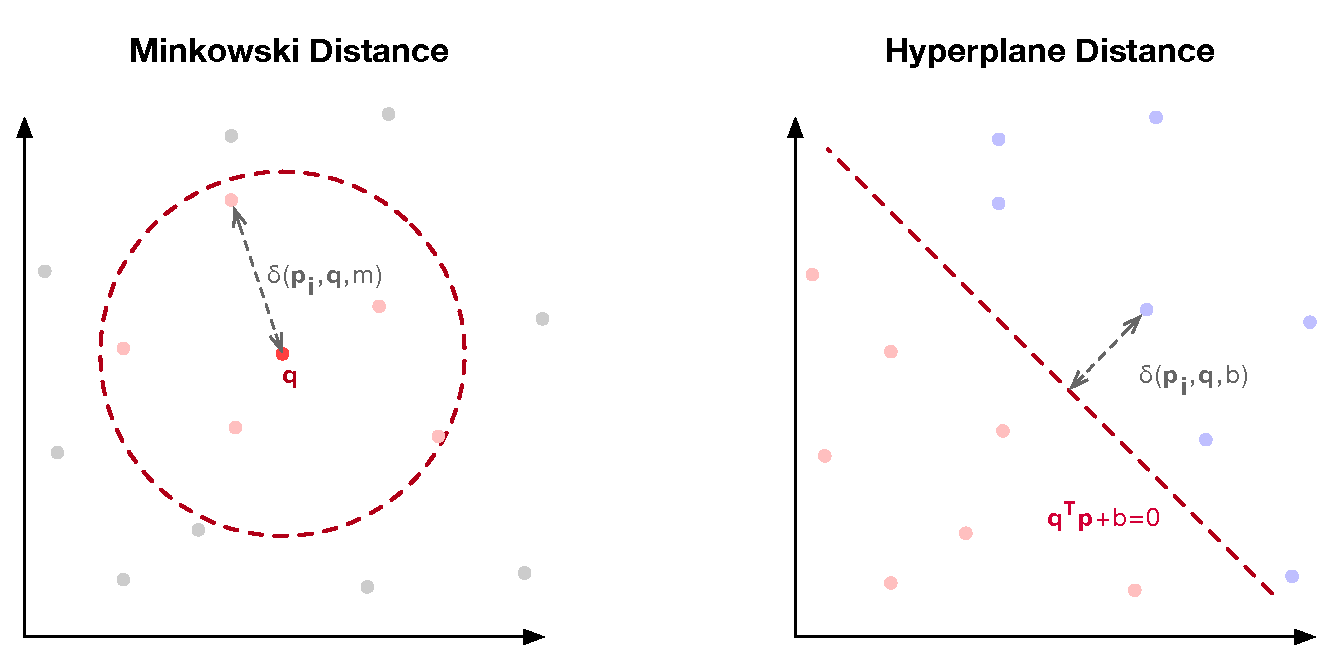
\includegraphics[width=\textwidth]{figures/distance_computations.eps}
    \caption{Two examples of distance functions that fall into the broader category of a \acrshort{dfc}. On the left, the point-distance between $q$ and $p_i$ and on the right, the distance between a hyperplane $q^Tx+b = 0$ and points $p_i$.}
    \label{figure:distance_computation}
\end{figure}

As an aside, we must address the role of dimensionality $dim$ in the case of data domains that are subsets of vector spaces, i.e.,  $\domain_q \subset \mathbb{R}^{dim}$ or $\domain_q \subset \mathbb{C}^{dim}$. One could argue, that the dimensionality of such a vector space can also be seen as a parameter of the \acrshort{dfc}. Irrespective of the merits such an argument might have, we consider the dimensionality of the vector space to be a strictly structural property of the underlying data domain $\domain_q$ and thus thightly coupled to the data type. This means, that dimensionality as well as the data type are well-defined and remain constant within a query.

\subsection{Extending the Relational Model}

Using \cref{definition:dfc}, one can now start to integrate \acrshort{dfc} into the relational data model. In line with~\cite{Giangreco:2018thesis}, we first assume  $\domainset$ -- the set system of data domains supported by the database -- to be extended by whatever data domain $\domain_q$ is required. Following that recipe, a \acrshort{dbms} can be extended to support every type of (mathematical) object that is useful for a given application, such as but not limited to $\mathbb{R}^{dim}$ or $\mathbb{C}^{dim}$. 

\paragraph{Extended Projection and DFCs}

We use the idea of an extended projection $\pi_{\mathcal{E}}$ -- as proposed by \cite{Gupta:1995Generalized,Garcia:2009Database} and introduced in \cref{section:relational_data_model} -- wherein $\mathcal{E}$ denotes a list of projection expressions $e$ that involve attributes $\attribute_i \in \relation$. That is, in addition to the simple projection onto attributes $\attribute_i$, an extended projection may also include the evaluation of literals or functions as expressed in \Cref{definition:extended_projection}. 

\begin{definition}[label=definition:extended_projection]{Extended Projection $\projection_\mathcal{E}$}{}
Let $\relation$ be a N-ary relation over attributes $\attribute \in \schema (\relation)$ with tuples $t \in \relation$. We call $\projection_\mathcal{E}$ an \emph{extended projection} with $M$ projection elements $e_i \in \mathcal{E}$,

\begin{equation*}
    \mathcal{E} = \{ e_1, e_2, \ldots e_M \}, \textrm{with} \: e_i \in \schema(\relation) \vee e_i \in \domain_i \vee e_i \in \mathbb{F}
\end{equation*}

where $\mathbb{F}$ if a set of functions $f_i \colon \domain_{1} \times \domain_{2} \ldots \domain_{M} \rightarrow \domain_{out}$ and $\domain_i \in \domainset$. In other words, $e_i$ can can be an attribute, a literal value or a function.

\begin{equation*}
    \projection_{\mathcal{E}}(\relation) =  \{ t\left[ \mathcal{E} \right] : t \in \relation \} \textrm{ with } t\left[ \mathcal{E} \right] = \bigcup_{e_i \in \mathcal{E}}
    \begin{cases} 
        t \left[ e_i \right] & \text{if } e_i \in \schema(\relation) \\
        e_i  & \text{if } e_i \in \domain_i \\
        e_i(t \left[ \mathcal{E}^{'} \right]) & \text{if } e_i \in \mathbb{F} \\
    \end{cases}
\end{equation*}

\end{definition}

It is to be noted, that the domain of every function $f_i \in \mathbb{F}$ is again, an implicit projection $t \left[ \mathcal{E}^{'}\right]$, where $\mathcal{E}^{'}$ contains all projection elements required as function argument. That way, function invocations can be nested arbitrarily. Furthermore, every function has access to all the attributes present in $\relation$.

If now we assume any DFC supported by the \acrshort{dbms} to be member of $\mathbb{F}$, the evaluation of a \acrshort{dfc} as part of a query can be expressed as follows:

\begin{definition}[label=definition:spf_rel]{\acrlong{dfc} in Extended Projection $\pi_{\mathcal{E}}$}{}
    Let $\symdfc \colon \domain_q \times \domain_q \times \domain_{1} \ldots \times \domain_{N-2} \to \mathbb{R}$ be a N-ary \acrshort{dfc}. The \emph{extended projection} $\pi_{\symdfc(a_1, a_2, \ldots a_N)}(\relation) \textrm { with } a_i \in \schema(\relation) \vee a_i \in \domain_i \vee a_i \in \mathbb{F}$ denotes the evaluation of $\symdfc$ using any number of argument. Applying $\pi_{\delta(\cdot)}$ on a M-ary relation $\relation$ introduces a new distance attribute $\mathcal{A}_\delta$, i.e., $\mathtt{SCH}(\pi_{\symdfc(\cdot), \mathcal{A}_1, \ldots \mathcal{A}_M}(\relation)) = \mathtt{SCH}(\relation) \cup \{ \mathcal{A}_\delta \}$
\end{definition}

Obviously, the evaluation of multiple \acrshort{dfc}s in a single, extended projection or the combination of simple attribute projections with the evaluation of \acrshort{dfc}s are also allowed. In fact, all of the following expressions are valid examples of the extended projection on relation $\relation$ with $\mathtt{SCH}(\relation) = \{ \mathcal{A}_1, \mathcal{A}_2, \mathcal{A}_3, \mathcal{A}_4 \}$ and $\delta_i = \mathtt{IMP}(\symdfc_i)$: 
\begin{enumerate*}[label=(\roman*)]
    \item Evaluation of multiple \acrshort{dfc}s with same or different probing arguments (e.g., $\pi_{\delta_1(\mathcal{A}_1), \delta_2(\mathcal{A}_1)}(\relation)$), 
    \item evaluation of same \acrshort{dfc} using same or different probing arguments (e.g., $\pi_{\delta_1(\mathcal{A}_1), \delta_1(\mathcal{A}_2)}(\relation)$),
    \item combination of \acrshort{dfc}s with any attribute projection and/or algebraic expression evaluation (e.g., $\pi_{\delta(\mathcal{A}_1), \mathcal{A}_2, \mathcal{A}_4}(\relation)$).
\end{enumerate*}

Consequently, the calculated distance becomes an explicit attribute in the relation $\relation$, which can then be used by downstream operators or system components using the \acrshort{dbms}. This makes sense, for example in \acrshort{nns}, because the distance obtained is usually converted to a similarity score by some correspondence function.

\paragraph{Ranked Relations}

To support sorting by the obtained distance (or any other attribute for that matter), which is an essential part of many types of proximity based queries, we use a variant of the \emph{ranked relation} as proposed by \cite{Chengkai:2005RankSQL} and described in \cref{section:rel_extensions}. A ranked relation $\rankedrel$ exhibits an ordering of tuples $t \in \rankedrel$, which is induced by $\mathcal{O}$. As opposed to \cite{Chengkai:2005RankSQL} and more in line with \cite{Garcia:2009Database}, we assume $\mathcal{O} \subset \schema (\relation)$ to be a sequence of \emph{attributes} by which the relation should be sorted,\footnote{We argue that formally, the evaluation of a \emph{scoring function}, as proposed by \cite{Chengkai:2005RankSQL}, can be expressed within the scope of the extended projection and does not need to be part of the order operation.} as is specified in \Cref{definition:ranked_relation}.

\begin{definition}[label=definition:ranked_relation]{Ranked relation $\rankedrel$}{}
Let $\relation$ be a N-ary relation over attributes $\attribute \in \schema (\relation)$ with $M$ tuples $t_m \in \relation$. We call $\rankedrel$ a \emph{ranked relation} with ranking attributes $\mathcal{O} \subset \schema (\relation)$. $\mathcal{O}$ induces a non-strict, total ordering using the binary, lexicographic ranking relation $\preceq$, such that:

\begin{gather*}
    t_i \preceq t_k  = \bigvee_{a \in \mathcal{O}} t_i \preceq_{a} t_k, \textrm{with} \\ 
    t_i \preceq_{a} t_k  \leftrightarrow t_i \left[ a \right] \leq t_k \left[ a \right]
\end{gather*}

The position of a tuple $t \in \rankedrel$ w.r.t. $\preceq$ is signified by the ranking function

\begin{equation*}
    \mathtt{RANK}: \relation \rightarrow \left[ 1, M \right]
\end{equation*}

which assigns a rank $r \in \left[ 1, M \right]$ depending on its position within $\rankedrel$, i.e., first elements gets rank $1$, second element rank $2$ etc.

\end{definition}

It is to be noted, that the ranking $\mathcal{O}$ is an inherent property of a ranked relation $\rankedrel$ as is, for example, its schema $\schema(\relation)$. That property is retained or induced as operators are being applied. Furthermore, if a relation does not exhibit a specific ordering, then $\mathcal{O}$ is empty and $\rankedrel = \relation^{\emptyset} = \relation$. Importantly, though, we expect an unordered relation to still exhibit some interal ordering of elements, which we call the \emph{natural ordering} of $\relation$ and which is not related to any observable property. Consequently, $\mathtt{RANK}$ is also defined for such relations, even though the returned values may appear arbitrary.

To explicitly order a relation, we introduce the \emph{relational order operator} $\order_{\mathcal{O}}$.

\begin{equation}
    \label{equation:rel_alg_tau}
    \order_{\mathcal{O}}(\relation) = \rankedrel
\end{equation}

For example, using the relation $\relation$ with $\mathtt{SCH}(\relation) = \{ \mathcal{A}_1, \mathcal{A}_2, \mathcal{A}_3, \mathcal{A}_4 \}$, the application of $\tau_{\attribute_1,\attribute_2}$ on relation $\relation$ sorts the tuples $t_i \in \relation$ based on $\attribute_1$ and breaks ties sorting by $\attribute_2$. Tuples equal in both attributes appear in an arbitrary order. We can use the duality property of the individual ranking relations to support ascending and descending order in an actual implementation.

\paragraph{k-selection}

To be able to execute a specific type of proximity based query -- namely, \acrshort{knn} or \acrshort{kfn} -- we require one last extension to the relational algebra in the form of the \emph{k-selection} operator $\limit(\relation)$, which simply limits the cardinality of a relation $\relation$ to the first $k$ tuples. It is trivial to see that for a ranked relation $\rankedrel$, $\lambda_k(\rankedrel)$ limits the tuples to the top $k$ results w.r.t. to the ordering induced by $\mathcal{O}$.

\begin{equation}
    \limit(\rankedrel) = \{ t \in \rankedrel \colon \mathtt{RANK}(t) \leq k \}
\end{equation}

We can now use \cref{example:rel_painting_w_features} to demonstrate the flexibility of the proposed algebra and the different types of queries that can be expressed through it.

\begin{example}[label=example:rel_painting_w_features]{Relation listing paintings with feature vectors}{}
    
    $\relation_{p}$ lists paintings with their title $\mathcal{A}_{t}$, the year of their creation $\mathcal{A}_{y}$ and some arbitrary feature vector $\mathcal{A}_{f}$. Note that $\domain_{f} \subset \mathbb{R}^{3}$.
        
    \begin{center}
        \begin{tabular}{ l || l | l | l |}
            $\relation_{p}$ & $\mathcal{A}_{t}$  & $\mathcal{A}_{y}$  & $\mathcal{A}_{f}$ \\ 
            \hline
            \hline
            $t_1$ & Mona Lisa & 1506 & $\left\lbrack 0.0, 0.2, -1.3 \right\rbrack$ \\
            \hline
            $t_2$ & The Starry Night & 1889 & $\left\lbrack 1.0, 0.9, 2.6 \right\rbrack$ \\
            \hline
            ... & ... & ... & ... \\
            \hline
            $t_N$ & Las Meninas & 1665 & $\left\lbrack -0.5, 3.0, 0.8 \right\rbrack$ \\
            \hline
        \end{tabular}
    \end{center}

    Using \acrshort{dfc}s and the proposed, relational algebra,  we can now express:

    \begin{center}
        \begin{tabular}{||l l r ||} 
         \hline
         Name & Result & Algebraic Form \\
         \hline\hline
         \acrshort{nns} / \acrshort{kfn} & $\relation^{\mathcal{A}_d\uparrow}$ & $\lambda_k (\tau_{\mathcal{A}_d\uparrow} ( \pi_{\mathcal{A}_{y}, \delta(\mathcal{A}_{f})}  ( \relation_p)))$  \\ 
         \hline
         \acrshort{fns} / \acrshort{knn}& $\relation^{\mathcal{A}_d\downarrow}$ & $\lambda_k (\tau_{\mathcal{A}_d\downarrow} ( \pi_{\mathcal{A}_{y}, \delta(\mathcal{A}_{f})}  ( \relation_p)))$   \\
         \hline
         $\epsilon$NN~\cite{Giangreco:2018thesis} & $\relation^{\mathcal{A}_d\uparrow}$ & $\tau_{\mathcal{A}_d\uparrow} ( \sigma_{\mathcal{A}_d \leq \epsilon} ( \pi_{\mathcal{A}_{y}, \delta(\mathcal{A}_{f})} ( \relation_p)) )$  \\
         \hline
         \acrshort{nns} w. selection & $\relation^{\mathcal{A}_d\uparrow}$ &  $\tau_{\mathcal{A}_d\uparrow} ( \pi_{\mathcal{A}_{year}, \delta(\mathcal{A}_{f})} ( \sigma_{\mathcal{A}_{y} = 1889} ( \relation_p)) )$\\
         \hline
         Multi order & $\relation^{\mathcal{A}_{d1}\uparrow,\mathcal{A}_{d2}\uparrow}$ & $\tau_{(\mathcal{A}_{d1}\uparrow,\mathcal{A}_{d2}\uparrow} ( \pi_{\delta_1(\mathcal{A}_{f}), \delta_2(\mathcal{A}_{f})}  ( \relation_p))$ \\ 
         \hline
         DFS \& aggregate & $\relation$ & \\ 
         \hline
        \end{tabular}
    \end{center}

\end{example}

\subsubsection{Algebraic Properties of  \texorpdfstring{$\pi_{\mathcal{E}}$}{Pi}, \texorpdfstring{$\order_{\mathcal{O}}$}{Tau}, \texorpdfstring{$\limit$}{Lambda}}

Since a query planner of a \acrshort{dbms} must be able to manipulate the operators that were introduced before, there is a series of algebraic properties that must be considered. For unary operators, we must consider \emph{commutativity}, i.e., whether changing the order of application leads to the same result or not. A unary operator $\mathtt{OP}$ commutes if, and only if, $ \mathtt{OP}_1 (\mathtt{OP}_2 ( \relation)) = \mathtt{OP}_2 (\mathtt{OP}_1 (\relation))$.

For binary operators, we must consider the \emph{commutativity of operands}, i.e., whether $\mathtt{OP} (\relation_L, \relation_R) = \mathtt{OP}(\relation_R, \relation_L)$. Furthermore, w.r.t. to unary operation, there is \emph{distributivity} to consider, i.e., whether $\mathtt{OP}_{1} (\mathtt{OP}_{2} (\relation_L,  \relation_R)) = \mathtt{OP}_{2} ( \mathtt{OP}_{1} ( \relation_L), \mathtt{OP}_{1} ( \relation_R))$. A summary of these properties can be found in \Cref{table:ext_algebraic_properties}.

To support ranked relations, we first an foremost require all existing, relational operators to be either \emph{order retaining} or \emph{order inducing}. It follows from its definition, that $\order_{\mathcal{O}}$ is an order inducing operator. Furthermore, $\selection$, $\projection$, $\rho$ and $\limit$ are order retaining, since they do not alter the input relation w.r.t ordering.

It is a bit more complicated for the binary operators, which do not behave consistently: On the one hand, the set difference ($\setminus$), the set intersection ($\cap$) and the natural join ($\Join_{\mathcal{P}}$) retain the order of the left operand $\relation_L$, since the operators retain or remove elements from $\relation_L$ based on their presence in $\relation_R$, without taking ordering into account. Consequently, the operands no longer commute.

The set union ($\cup$) and the cross product ($\times$), on the other hand, combine two relations $\relation_L$ and $\relation_R$. The resulting relation does not have an order that can be expressed in the proposed framework and must thus be considered unordered, i.e., the operators are order inducing in that they induce a new, natural order.

\begin{table}
    \caption{The relational operators and their properties w.r.t to the proposed extensions.}
    \label{table:ext_algebraic_properties}
    \begin{tabular}{| l | c | c | c | c | c |}
        \hline
       \textbf{Name} & \textbf{Symbol} & \textbf{Arity} & \textbf{Order} & \textbf{Commutativity} & \textbf{Distributivity}\\ 
        \hline
        \hline
        Union & $\relation_{L}^{\mathcal{O}_1} \cup \relation_{R}^{\mathcal{O}_2}$ & 2 & $\emptyset$ & - &\\
        \hline
        Intersection & $\relation_{L}^{\mathcal{O}_1} \cap \relation_{R}^{\mathcal{O}_2}$ & 2 & $\mathcal{O}_{1}$ & - &\\
        \hline
        Difference & $\relation_{L}^{\mathcal{O}_1} \setminus \relation_{R}^{\mathcal{O}_2}$  & 2 & $\mathcal{O}_{1}$ & - &\\
        \hline
        Cartesian Product & $\relation_{L}^{\mathcal{O}_1} \times \relation_{R}^{\mathcal{O}_2}$ & 2 & $\emptyset$ & - &\\
        \hline
        Natural Join & $\relation_{L}^{\mathcal{O}_1} \Join_{\mathcal{P}} \relation_{R}^{\mathcal{O}_2}$ & 2 & $\mathcal{O}_{1}$ & - &\\
        \hline
        Rename & $\rho_{\attribute_\mathtt{A} \rightarrow \attribute_\mathtt{B}}(\rankedrel)$ &  1 & $\mathcal{O}$ & $\projection$, $\selection$, $\rho$, $\limit$, $\order$ & $\cup$, $\cap$, $\setminus$, $\times$, $\Join$\\
        \hline
        Selection & $\selection_{\mathcal{P}}(\rankedrel)$ &  1 & $\mathcal{O}$ & $\projection$, $\selection$, $\rho$, $\order$ & $\cup$, $\cap$, $\setminus$, $\times$, $\Join$\\
        \hline
        Extended Projection & $\projection_{\mathcal{E}}(\rankedrel)$ &  1 & $\mathcal{O}$ & $\projection$, $\selection$, $\rho$, $\limit$, $\order$ & $\cup$, $\cap$, $\setminus$, $\times$, $\Join$\\
        \hline
        Limit & $\limit(\rankedrel)$ & 1 & $\mathcal{O}$ & $\projection$, $\rho$ & - \\
        \hline
        Order & $\order_{\mathcal{O}}(\relation^{\mathcal{O}^{'}})$ & 1 & $\mathcal{O}$ &  $\projection$, $\selection$, $\rho$ & $\cap$, $\setminus$, $\Join$\\
        \hline
    \end{tabular}
\end{table}

When turning to the individual operators, the extended projection $\projection_\mathcal{E}$ inherits all its properties from the normal projection $\projection$ if we require $f \in \mathbb{F}$ to be side-effect free, i.e., it must not influence the state of the \acrshort{dbms} in any other way than producing the desired output.

The order operator $\order_{\mathcal{O}}$ commutes with other unary operators if they are neither \emph{rank sensitive} nor \emph{rank inducing}, namely, $\projection$, $\selection$ and $\rho$.

\begin{equation*}
    \order_{\mathcal{O}^{'}}(\order_{\mathcal{O}}(\relation)) \neq \order_{\mathcal{O}}(\order_{\mathcal{O}^{'}}(\relation)) \\
\end{equation*}

In addition, distributivity with all the order retaining binary operations is given, e.g., when taking set intersection as an example.

\begin{equation*}
    \order_{O} (\relation_L^{O_L} \cap \relation_R^{O_R}) = \order_{O} (\relation_L^{O_L}) \cap \order_{O} (\relation_R^{O_R})) = (\relation_L \cap \relation_R)^{O}
\end{equation*}

However, the order operator does not distribute with the order inducing, binary operators $\cup$ and $\times$, for example, taking set union as an example.

\begin{equation*}
    \order_{O} (\relation_L^{O_L} \cup \relation_R^{O_R}) = (\relation_L^{O_L} \cup \relation_R^{O_R})^{O} \stackrel{!}{\neq} \order_{O} (\relation_L^{O_L}) \cup \order_{O} (\relation_R^{O_R})) = (\relation_L \cup \relation_R)^{\emptyset}
\end{equation*}

The k-selection operator $\limit$ does neither commute with the selection operator $\selection$ nor the order operator $\order$.

\begin{gather*}
    \limit(\order(\relation)) \neq \order(\limit(\relation)) \\
    \limit(\selection(\relation)) \neq \selection(\limit(\relation)) 
\end{gather*}

Lack of commutativity $\limit$ with $\order$ follows directly from its definition: $\limit$ is sensitive to the ranking of a $\rankedrel$ and $\order$ influences that ranking. Consequently, executing $\limit$ before or after sortings will yield different results. For $\selection$, one can turn to \Cref{proof:limit_non_commutativity}.


\begin{proof}[label=proof:limit_non_commutativity]{Non-commutativity of $\selection$ and $\limit$}{}
    Let $\relation$ be a relation with $M$ rows and $\schema(\relation) = \{ \attribute_R \}$ and let further be $t \left[ \attribute_R \right] = \texttt{RANK} (t) \forall t \in \relation$. If $\selection$ and $\limit_k$ were to commute, then 

    \begin{equation*}
        \selection_{\attribute_R > M - 2} (\limit_{M-1} (\relation)) = \limit_{M-1} (\selection_{\attribute_R > M - 2}(\relation))
    \end{equation*}

    However, we can proof by contradiction that this does not hold since:

    \begin{equation*}
        \selection_{\attribute_R > M - 2} (\limit_{M-1} (\relation)) = \{ t_M \} \stackrel{!}{\neq} \limit_{M-1} (\selection_{\attribute_R > M-2}(\relation)) = \{ t_{M-1}, t_M \}
    \end{equation*}

    That is, whenever $\limit_k$ removes tuples that match the predicate of $\selection$, the order of execution influences the result and the two operators do not commute.
\end{proof}

\subsection{\texorpdfstring{\acrshort{dfc}s}{DFCs} and Query Planning}
\label{section:dfc_and_planning}

In addition to the algebraic properties of the extended relational algebra, we can also leverage the requirements imposed on the structure of a function $f \in \mathbb{F}$ to enable a \acrshort{dbms} to plan and optimize the execution of a proximity based query by altering the execution plan in terms of \acrshort{dfc} implementations that should be employed. To do so, we propose the notion of a \emph{function hierarchy} depicted in \Cref{figure:function_hierarchy}. As we move down that hierarchy, more information about the structure of a function and the concrete implementation employed in query plan becomes available to the \acrshort{dbms}. That information can be leveraged when deciding about the best execution path:

\begin{figure}[bt]
    \centering
    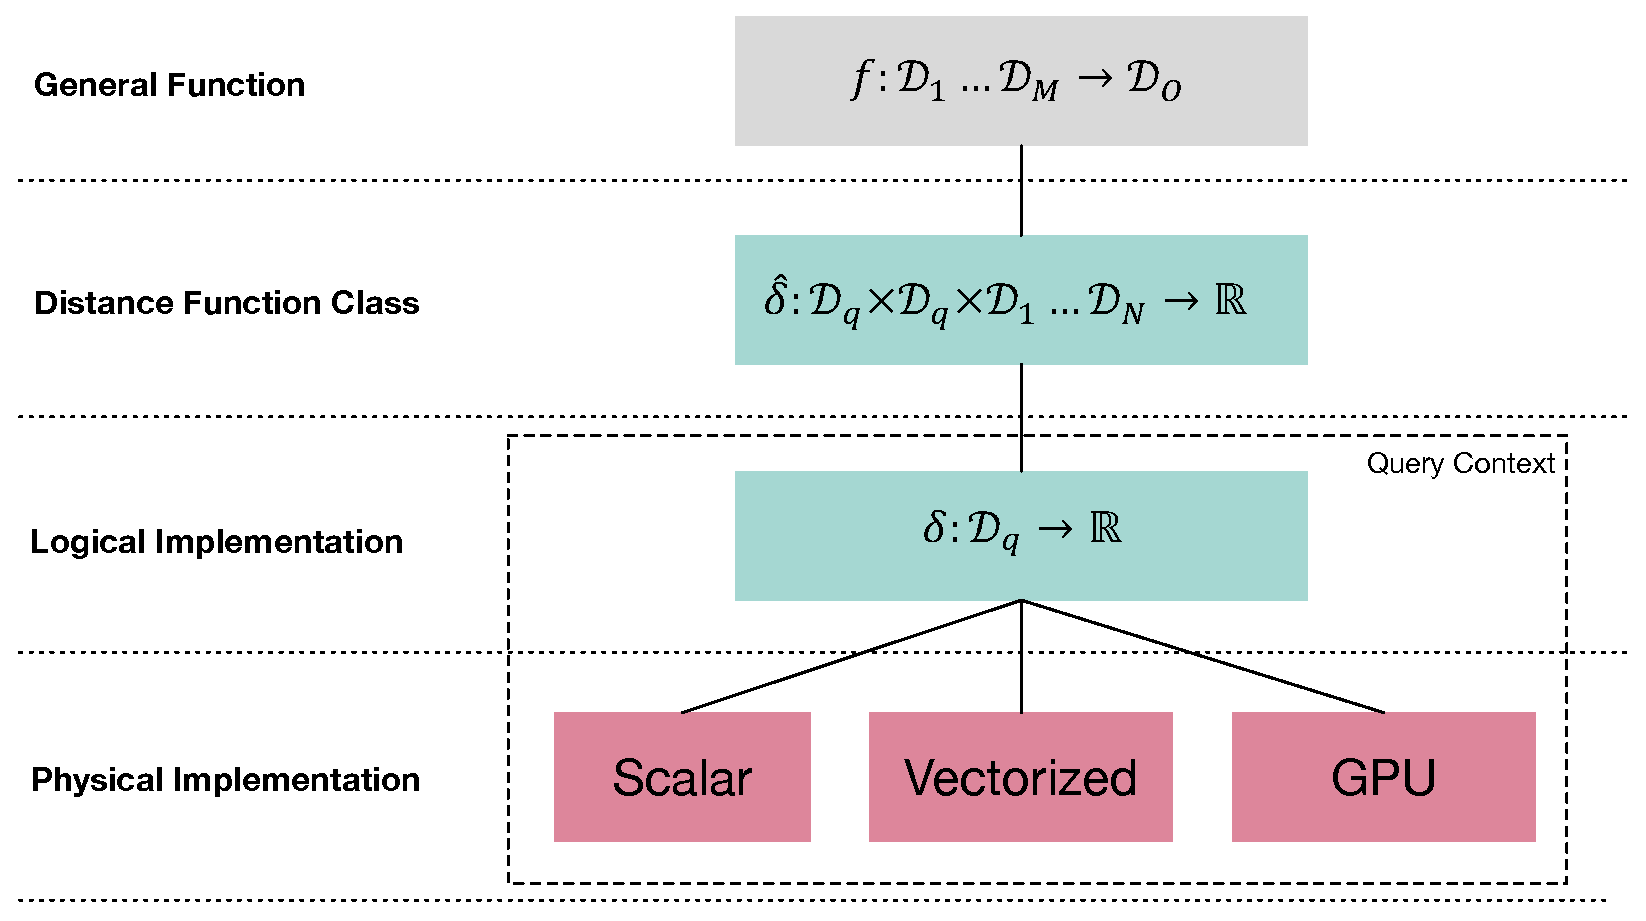
\includegraphics[width=\textwidth]{figures/function_hierarchy.eps}
    \caption{Function hierarchy of all $f \in \mathbb{F}$. As we go down the hierarchy, the \acrshort{dbms} gains knowledge about a function's structure.}
    \label{figure:function_hierarchy}
\end{figure}

\begin{description}
    \item[General Function] Every function $f \in \mathbb{F}$ -- even user-defined ones -- is known beforehand with information about its domain and co-domain. This allows to provide optimised implementations, e.g., for the different data domains, to avoid type casting during query exection.
    \item[Distance Function Class] Since DFCs constitute a specific type of function, we can embedd equivalences between a DFC and different types of high-dimensional index structures. Those equivalences allow a query planner to select one over the other, for a particular plan.
    \item[Logical Implementation] As an implementation of a query manifests, the structure of a DFC may change through implementation. For example, certain attributes may turn-out to remain constant, which can be leveraged by the planner to optimise execution.
    \item[Physical Implementation] As the physical execution plan emerges, a plan can make decisions as to what type of implementation for a DFC should be selected. For example, it may select a vectorised version of a DFC, which leverage \acrfull{simd} instructions of the CPU, over a scalar implementation that calculates the distance in a tight loop.
\end{description}

One identity that is particularly relevant for the execution of proximity based queries is the relationship between the execution of a DFC and a high-dimensional index. While there are many different types of HD-indexes, we distinguish between three broader categories proposed by \cite{Lejsek:2018Transactional} and introduced and discussed in \Cref{chapter:theory_multimedia_analysis_and_retrieval}, namely \emph{quantization based} (e.g., \acrshort{pq} or \acrshort{vaf}), \emph{hash based} (e.g., \acrshort{lsh} or \acrshort{sh}) and \emph{tree based} indexes. With respect to these classes, we postulate the relationship between an index and a DFC as given in \Cref{definition:dfc_and_index}. 

\begin{definition}[label=definition:dfc_and_index]{DFCs and high-dimensional index structures (exact case).}{}
    Let $\symdfc \colon \domain_q \times \domain_q \times \domain_{1} \ldots \times \domain_{n} \to \mathbb{R}$ be a \acrshort{dfc} and $\projection_{\mathcal{E}}$ be the extended projection involving execution of that DFC, i.e., $\symdfc \in \mathcal{E}$. A high-dimensional index $\mathtt{INDEX}$ is a pre-computed database object such that $\projection_{\symdfc(\cdot)}(\relation) = \mathtt{INDEX}(\relation)$ and therefore, 

    \begin{equation}
        \projection_{\mathcal{E}} (\relation) = \projection_{\mathcal{E} \setminus \symdfc} (\relation) \Join \mathtt{INDEX} (\relation)
    \end{equation}
    
    We call such an index \emph{exact} and we can use it as a replacement for the DFC.
\end{definition}

In practice, this equivalemce is a property of a particual index instance and can be stored as metadata in the \acrshort{dbms} catalogue. Furthermore, there may be some implementation-specific restrictions to \Cref{definition:dfc_and_index}.

\begin{itemize}
    \item Indexes are always derived from a materialized relation $\relation$ and a feature attribute 
    $\attribute_f \in \schema(\relation)$, Therefore, an index can only replace a DFC if they operate on an unaltered version of $\attribute_f$. Changes to $\attribute_f$, e.g., through application of another function, will render the index unusable for that query.
    \item Indexes are usually trained for a specific distance function (e.g., Euclidean) or class of distance functions (e.g., Minkowski). Therefore, an index can only replace a DFC if that DFC coincides with that function (-class).
    \item Hash-based indexes, by the very way they function, are only suitable replacements if the evaluation of the DFC is followed by an order and a k-selection operator.
\end{itemize}

With \Cref{definition:dfc_and_index} and those three boundary conditions, we have defined the basic relationship and rule that can be applied by a \acrshort{dbms}, when deciding whether or not to use a particular high-dimensional index structure.

\pagebreak


\section{Cost Model for Retrieval Accuracy}
Describe cost model for execution plans with following properties:

\begin{itemize}
    \item Cost as a function of atomic costs: $f(a_{cpu}, a_{io}, a_{memory}, a_{accuracy}) \longrightarrow C$
    \item Means to estimate results accuracy and associated considerations from execution path (e.g., when using index) based on properties of the index
    \item Means to specify importance of accurate results (e.g., global, per-query, context-based i.e. when doing 1NN search) in comparison to other factors
    \item Systems perspective 1: How can such a cost model be applied during query planning and optimization?
\end{itemize}

\section{Adaptive Index Management}

\begin{figure}[h!]
    \centering
    \begin{subfigure}[b]{0.40\textwidth}
        \centering
        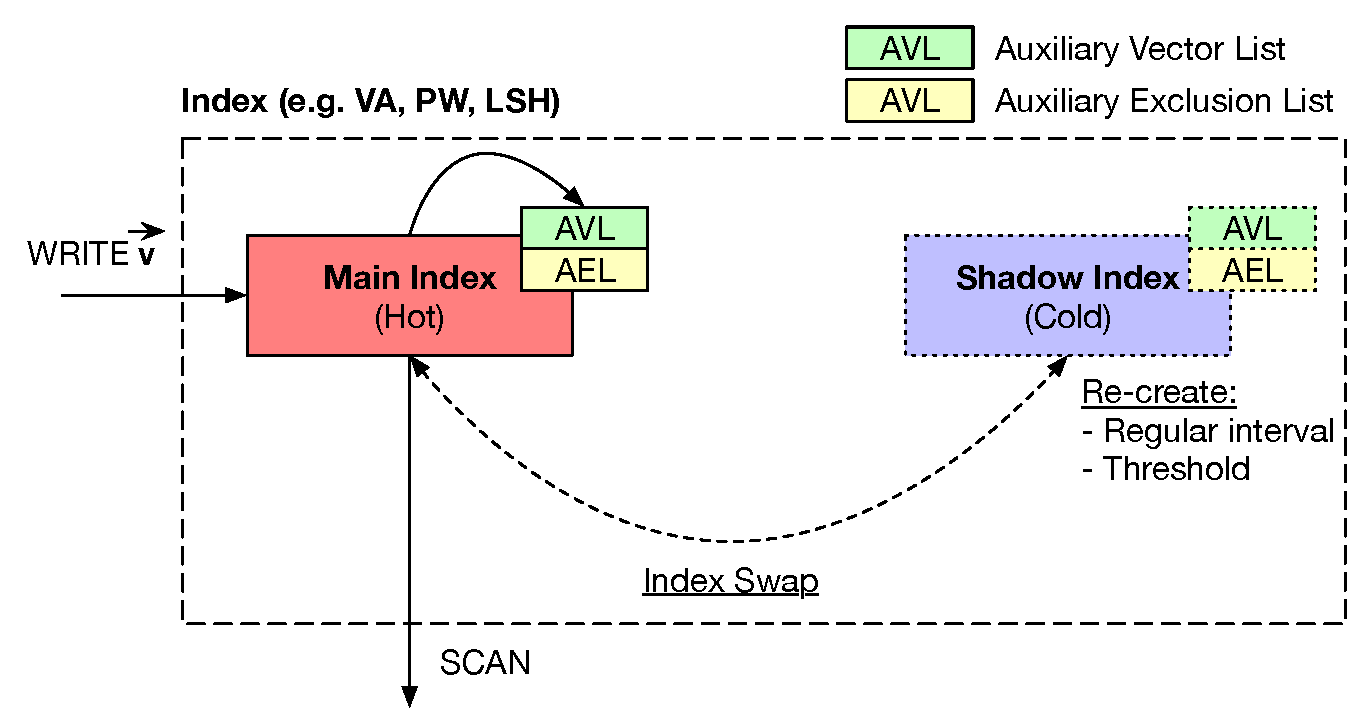
\includegraphics[width=\textwidth]{figures/adaptive_index.eps}
        \label{fig:adaptive_index:architecture}
    \end{subfigure}
    \hfill
    \begin{subfigure}[b]{0.40\textwidth}
        \centering
        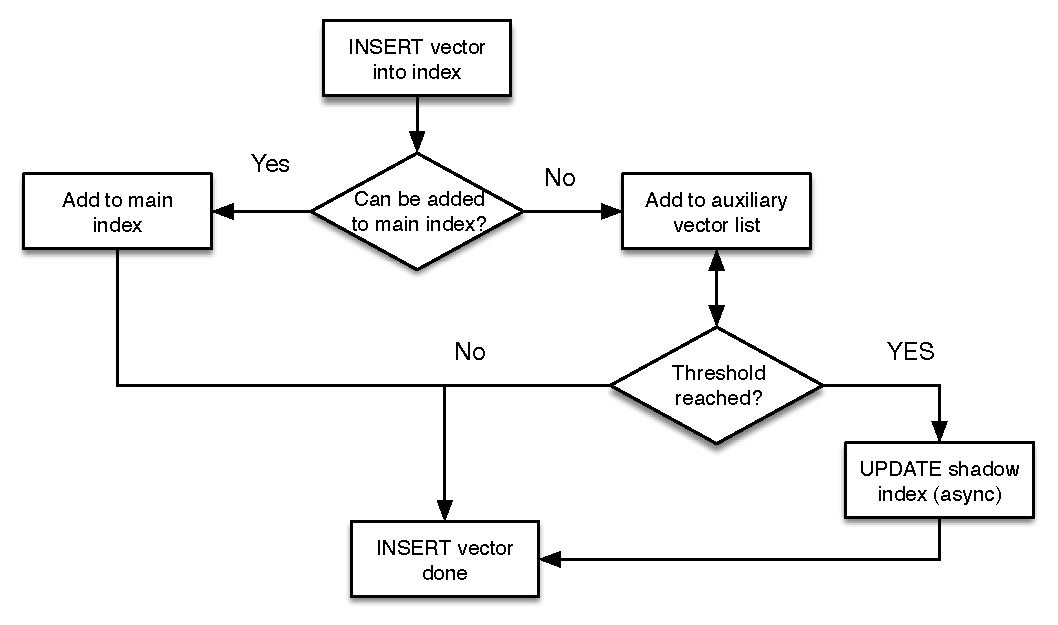
\includegraphics[width=\textwidth]{figures/adaptive_index_flow.eps}
        \label{fig:adaptive_index:flow}
    \end{subfigure}
    \caption{Adaptive index structures overview.}
    \label{fig:adaptive_index}
\end{figure}

Describe model for index management in the face of changing data (adaptive index management):

\begin{itemize}
    \item Reason about properties of secondary indexes for NNS (e.q., PQ, VA, LSH) with regards to data change
    \item Derivation of error bounds possible (e.g., usable for planning)?! Use in query planning?
    \item Systems perspective 1: How to cope with ``dirty'' indexes? Proposal: hot vs. cold index, auxilary data structure, offline optimization, see \cref{fig:adaptive_index}
    \item Systems perspective 2: On-demand index based on query workload?
\end{itemize}

\section{Architecture Model}

\todo[inline]{Putting everything together into a unified systems model (base on previous work + aforementioned aspects).}




